%%%%%%%%%%%%%%%%%%%%%%%%%%%%%%%%%%%%%%%%%%%%%%%%%%%%%%%%%%%%%%%%%%%%%%%
% BAB 2
%%%%%%%%%%%%%%%%%%%%%%%%%%%%%%%%%%%%%%%%%%%%%%%%%%%%%%%%%%%%%%%%%%%%%%%

\mychapter{2}{BAB 2 LANDASAN KEPUSTAKAAN}



\section{Tinjauan Pustaka}

% comments
%% comments
Beberapa referensi digunakan dalam penelitian ini. Pramukantoro dan Gofuku (\citeyear{pramukantoroHeartbeatClassifierContinuous2022}) dalam penelitiannya telah mengusulkan beberapa algoritma untuk melakukan klasifikasi detak jantung. Algoritma tersebut menggunakan RR-Interval dengan 9 deskriptor sebagai fiturnya. Penelitian tersebut menggunakan metode \textit{machine learning Decision Tree, Gradient Boosting, k-Nearest Neighbors, Multi-layer Perceptron, Random Forest}, dan \textit{Support Vector Machine}, serta model \textit{deep learning Artificial Neural Network} (ANN). Penelitian tersebut mencapai nilai akurasi 99,31\% dengan menggunakan metode \textit{decision tree}, serta teknik \textit{random oversampling} untuk menambah jumlah sampel. Selain itu, penelitian tersebut juga melakukan eksperimen implementasi inferensi secara \textit{realtime} untuk memprediksi kesehatan pasien dan mencapai hasil yang baik.

Pada penelitian lain, \textcite{mondejar-guerraHeartbeatClassificationFusing2019} mengusulkan algoritma klasifikasi detak jantung dengan menggunakan fitur RR-Interval dengan 8 deskriptor. Dengan menggunakan fitur RR-Interval dan metode SVM, penelitian tersebut mendapatkan nilai akurasi 76,2\%. Penelitian tersebut juga menggunakan metode \textit{ensemble} SVM dengan fitur gabungan RR-Interval, wavelet, dan \textit{higher order statistics} (HOS) dan mendapat nilai akurasi 94,5\%.

\section{Landasan Teori}


\subsection{\emph{Electrocardiogram} (ECG)}
\label{subsec: landasan-ecg}

\textit{Electrocardiogram} (ECG) merupakan uji kardiologi yang umum dilakukan untuk merekam aktivitas listrik jantung selama suatu periode dengan menggunakan elektroda \parencite{yoonDeepLearningbasedElectrocardiogram2019}. Elektroda tersebut mendeteksi perubahan listrik kecil yang disebabkan oleh depolarisasi dan repolarisasi otot jantung pada tiap detaknya. Hasil dari ECG tersebut berupa gelombang yang dapat digunakan untuk diagnosis medis. ECG dapat digunakan untuk berbagai tujuan, seperti mengukur konsistensi, ukuran, dan lokasi denyut jantung serta untuk mengidentifikasi kerusakan jantung. 

Gambar \ref{fig: ecg-morphology} menunjukkan morfologi gelombang ECG. ECG terdiri dari beberapa komponen: gelombang P, kompleks QRS, dan gelombang T, serta durasi antara komponen tersebut \parencite{anbalaganAnalysisVariousTechniques2023}.  Gelombang P menunjukkan depolarisasi atrium, kompleks QRS menunjukkan depolarisasi ventrikel, dan gelombang T menunjukkan repolarisasi ventrikel.

\begin{figure}[h!]
  \centering
  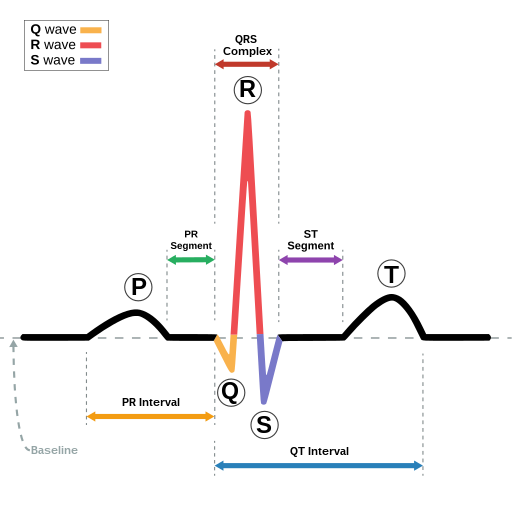
\includegraphics[width=.5\linewidth]{img/ecg-morphology.png}
  \caption{Morfologi gelombang ECG}
  Sumber: \textcite{wiki:xxx}
  \label{fig: ecg-morphology}
\end{figure}

\subsection{\textit{Long Short-Term Memory} (LSTM)}
\label{subsec: landasan-lstm}

\textit{Long Short-Term Memory} atau dapat disingkat LSTM merupakan pengembangan dari metode \textit{deep learning Recurrent Neural Network} (RNN). LSTM dirancang untuk mengatasi salah satu masalah yang umum terjadi pada RNN tradisional, yaitu hilangnya informasi masa lalu \parencite{hochreiterLongShorttermMemory1997}. Metode LSTM dapat diterapkan pada klasifikasi, pengolahan, dan prediksi berdasarkan data sekuensial, seperti teks dan suara,  termasuk juga data yang terkait dengan bidang kesehatan.

\begin{figure}[H]
  \centering
  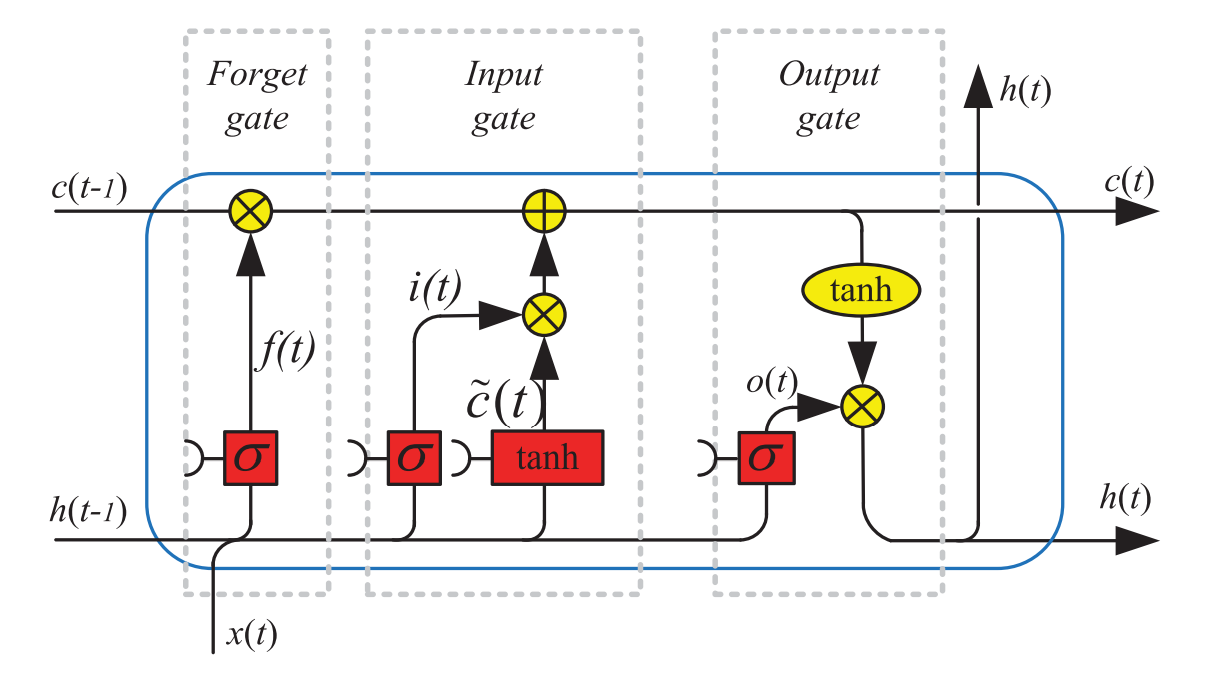
\includegraphics[width=.7\linewidth]{img/ecg-arch.png}
  \caption{Arsitektur sel LSTM}
  Sumber: \textcite{yuReviewRecurrentNeural2019}
  \label{fig:arsitektur-lstm}
\end{figure}

Gambar \ref{fig:arsitektur-lstm} menunjukkan arsitektur sel LSTM. Sebuah sel LSTM umumnya terdiri dari tiga buah \textit{gate}, yaitu \textit{input gate, output gate}, dan \textit{forget gate}. Ketiga gate tersebut berfungsi untuk mengatur informasi yang masuk maupun keluar dari sel LSTM.
\textit{Input gate} menentukan informasi baru yang akan disimpan pada \textit{cell state} (Ct), \textit{output gate} menentukan informasi apa yang akan jadi output, dan \textit{forget gate} menentukan informasi apa yang akan dibuang dari \textit{cell state} \parencite{yuReviewRecurrentNeural2019}.

Berdasarkan gambar \ref{fig:arsitektur-lstm}, secara matematis LSTM dapat didefinisikan dengan persamaan \ref{def-lstm}.
\begin{equation}
\begin{split}
    f_t &= \sigma (W_{fh}h_{t-1} + W_{fx}x_t + b_f), \\
    i_t &= \sigma (W_{ih}h_{t-1} + W_{ix}x_t + b_i),\\
    \tilde{c}_t &= \tanh (W_{\tilde{c}h}h_{t-1} + W_{\tilde{c}x}x_t + b_{\tilde{c}}), \\
    c_t &= f_t \cdot c_{t-1}+ i_t \cdot \tilde{c}_t,\\
    o_t &= \sigma (W_{oh}h_{t-1} + W_{ox}x_t + b_o), \\
    h_t &= o_t \cdot \tanh(c_t).
\end{split}
    \label{def-lstm}
\end{equation}
\noindent
Di mana \(f_t\), \(i_t\), \(o_t\) dan \(c_t\) masing-masing menunjukkan nilai \emph{forget gate}, \emph{input gate}, \emph{output gate}, dan \emph{cell state}.

% \subsection{Raspberry Pi 3}
% \label{subsec: landasan-raspi}
%
% %raspi secara umum
% Raspberry Pi merupakan sebuah komputer mini seukuran kartu kredit yang dikembangkan oleh Raspberry Pi Foundation \parencite{8756967}. 
% Raspberry Pi memiliki beberapa kelebihan, seperti ukurannya yang kecil, konsumsi daya yang rendah, harga yang terjangkau, serta kemampuan komputasi baik.
% %need citation
% Raspberry Pi dapat diaplikasikan pada berbagai bidang, seperti industri, agrikultur, bioteknologi, dan kesehatan \parencite{9760691}.
%
% %raspi 4 
% %*sekara sudah bukan yang terbaru, sudah ada raspi 5
% % Raspberry Pi 4 model B merupakan salah satu varian dari Raspberry Pi generasi keempat. Raspberry Pi 4 model B memiliki spesifikasi prosesor \textit{quad-core} ARM Cortex-A72 1.5GHz, dengan pilihan RAM 2GB, 4GB, atau 8GB LPDDR4-3200 SDRAM. Raspberry Pi 4 model B juga dilengkapi dengan konektivitas WiFi 2.4GHz dan 5GHz, Bluetooth 5.0, serta \textit{ethernet} dengan kecepatan maksimum 1Gbps. Raspberry Pi 4 model B juga memiliki \textit{port micro} HDMI, USB 3.0, USB 2.0, dan port GPIO.
%
% % raspi 3
% % Pengujian dilakukan pada perangkat Raspberry Pi 3B. Perangkat ini memiliki prosesor ARMv8 quad-core 1,2GHz dan RAM 1GB LPDDR2. Konektivitas perangkat ini didukung dengan 2.4Ghz WiFi serta \textit{ethernet} dengan kecepatan maksimum 100Mbps.
% Raspberry Pi 3 merupakan salah satu varian dari Raspberry Pi generasi ketiga. Raspberry Pi 3 memiliki spesifikasi prosesor ARMv8 \textit{quad-core} 1,2GHz dan RAM 1GB LPDDR2. Raspberry Pi 3 juga telah dilengkapi dengan konektivitas WiFi 2.4GHz dan \textit{ethernet} dengan kecepatan maksimum 100Mbps. Raspberry Pi 3 juga memiliki \textit{port} HDMI, USB 2.0, dan \textit{port} GPIO.

% klasifikasi detak jantung
% tentang detak jantung menurut AAMI

% heart related disease class
% N, sveb, veb, f, dan q
\section{Ke}

% metrik evaluasi
% akurasi, presisi, recall, f1-score

% TODO
% landasan teori lain
